\documentclass[11pt, oneside]{article}   	% use "amsart" instead of "article" for AMSLaTeX format
\usepackage[margin=1in]{geometry}                		% See geometry.pdf to learn the layout options. There are lots.
\geometry{letterpaper}                   		% ... or a4paper or a5paper or ... 
%\geometry{landscape}                		% Activate for rotated page geometry
\usepackage[parfill]{parskip}    		% Activate to begin paragraphs with an empty line rather than an indent
\usepackage{graphicx}				% Use pdf, png, jpg, or eps§ with pdflatex; use eps in DVI mode
								% TeX will automatically convert eps --> pdf in pdflatex		
\usepackage{amssymb}
\usepackage{tcolorbox}
\usepackage{url}

\usepackage{amsmath}
%SetFonts
%\usepackage{multicolumn}
\usepackage{multirow}
%SetFonts


\title{Homework 3}
\author{CS 4364/5364\\Spring 2022}
\date{Due: 23 February 2022}							% Activate to display a given date or no date

\begin{document}
\maketitle

%Because of the reliance of the particular assignments in this class on mathematical notation, 
%and the fact that all assignments will be submitted electronically, 
%students are encouraged to use \LaTeX{} to formalize their responses. 
%\textbf{For those enrolled in the graduate section the use of latex is \emph{required}.}
%This assignment (like all others) will be posted on the course \texttt{github}\footnote{\url{github.com/deblasiolab/CS4364-documents}} as source code as well as in PDF form on the course website. 
%Please submit your assignment to the professor via email, either as a link to your assignment online (i.e. overleaf or github) or as an attachment. 
%Graduate students will need to include the \texttt{.tex} files as well as a PDF, this is optional but encouraged for undergraduates. 

\begin{enumerate}
\item \textbf{(25 points)} 
\textbf{\emph{Profile Alignment Problem} Given two sequence profiles $T$ and $S$,  of sizes $\sigma \times n$ and $\sigma \times m$ respectively 
(that is each represents a sequence of length $n$ [$m$], but with probabilities of each character from the alphabet at each position), 
determine the optimal alignment (i.e. which columns of $S$ align with which columns of $T$) under the scoring scheme $\delta$.}

\textbf{Your task: \textbf{modify} the Needlman-Wunch global alignment algorithm to consider these profiles rather than sequences. 
You can assume that the replacement costs are defined in a function $\delta(a,b) \rightarrow \mathbb{Z} , \forall a,b \in \Sigma \cup \{'-'\}$.
Give the algorithm, an explanation of correctness, and analysis of it's running time. }

\textbf{An example alignment is shown below over the alphabet $\Sigma=\{\texttt{A},\texttt{C},\texttt{T},\texttt{G}\}$, as well as it's alignment score. 
Note that the score for a column is now no longer the value of $\delta$ for the two characters being aligned, but the weighted sum of these values.}


\begin{figure}[h!] %DONT USE THE [h!] PART UNLESS YOU REALLY NEED TO!! (Do as I say, not as I do)
\begin{centering}
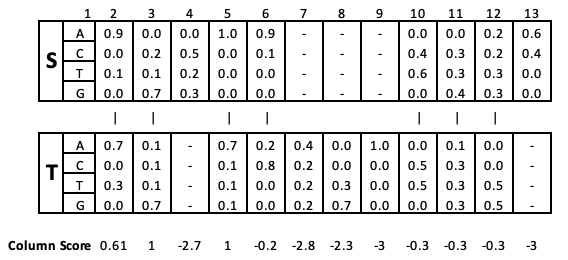
\includegraphics{HW3_Align}
\caption{Alignment of two profiles}
\end{centering}
\end{figure}

\begin{figure}[h!]
\begin{centering}
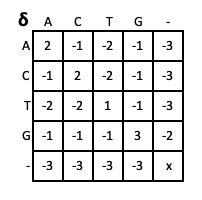
\includegraphics{HW3_Delta}
\caption{Scoring scheme}
\end{centering}
\end{figure}

{\huge Solution}\\
{\Large the algorithm}
\begin{itemize}
\item Let there be a function $M:\mathbb{R}^\sigma\times\mathbb{R}^\sigma\times\mathbb{R}^{\sigma\times\sigma}\rightarrow\mathbb{R}$ 
which takes as input two profiles (real-valued vectors of length $\sigma$) 
and a delta function (a real-valued $\sigma\times\sigma$ matrix) 
then returns the cost of aligning the two columns under the delta function. 
 Define it as follows:
 \[
 	M(A,B,\delta) := \sum_{a,b\in\Sigma} A[a]*B[b]*\delta(a,b).
 \]
 \item Let there be two other functions of a similar type; 
 $I:\times\mathbb{R}^\sigma\times\mathbb{R}^{\sigma\times\sigma}\rightarrow\mathbb{R}$ and 
 $D:\times\mathbb{R}^\sigma\times\mathbb{R}^{\sigma\times\sigma}\rightarrow\mathbb{R}$ that provide the score of inserting or deleting a profile respectively. 
 Define them as: 
  \[
 	I(B,\delta) := \sum_{b\in\Sigma} B[b]*\delta('\texttt{-}',b),
 \] 
 and
  \[
 	D(A,\delta) := \sum_{a\in\Sigma} A[a]*\delta(a,'\texttt{-}').
 \]
 \item Alter the recurrence relation from Needlman-Wunsch to consider these new scores as follows, 
 assuming we can represent each sequence of profiles such that the first dimension is the position in the sequence and the second is the frequency of a character:
 \[
 \begin{array}{rl}
 V(i,j) = \max &
 
 \begin{cases}
V(i-1,j-1) + M(S[i],T[j],\delta) & // \text{align positions $i$ and $j$ from } \\
					   & // \text{$S$ and $T$ respectively} \\
V(i-1,j) + D(S[i],\delta)	   & // \text{delete position $i$ from $S$}\\
V(i,j-1) + I(T[j],\delta)	   & // \text{insert position $j$ from $T$}\\
 \end{cases}
 \end{array}
 \]
 \item Initialize the $V$ matrix as follows:
 \[
 	\begin{array}{ll}
	V(0,0) = 0 & \\
	V(i,0) = V(i-1,0) + D(S[i]) & 1 \le i \le n\\
	V(0,i) = V(0,i-1) + I(T[j]) & 1 \le i \le m\
	\end{array}
 \]
 \item Fill in the remaining parts of $V$ table and perform traceback as described in the original algorithm outputting profiles instead of single characters in the alignment. 
\end{itemize}
\end{enumerate}


{\Large correctness}\\
The initializations match the original initializations in that the best alignment between any string and the empty string is to remove (insert/delete) 
all of the characters up to this point (this is the only choice)
The choice made in the recurrence relation is still to decide on what the last column should be in the optimal alignment between the prefixes $S[1...i]$ and $T[1....j]$, 
thus as long as the previous steps provide the optimal scores you can intuition though in a inductive manner to show each step is then correct. 
Since we know the base cases (initializations) are true, it follows that the best alignment score of the full sequences will be held in $V(n,m)$ as in the original algorithm. 
Because the paths are the same as in the original algorithm with respect to how to output matches/mismatch, insertion, and deletion columns
we know the traceback will output the correct alignment in line with the example. 

{\Large run-time analysis}\\
the first two bullets are simply definitions, and thus have no running time. 
The initialization fills in $n+m+1$ cells of the table, and from the definition we can see that calculating both $I$ and $D$ take $O(\sigma)$ time. 
Therefore, the total running time of the initializations is $O\left(\sigma\left(m+n\right)\right)$.
Filling in the table still means calculating values for $n\times m$ values, but at each cell we must run $M$, $I$, and $D$ which take $O(\sigma^2)$, $O(\sigma)$, and $O(\sigma)$ time respectively. 
This means calculating the value at each cell is $O(\sigma^2)$-total time, 
and thus filling in $V$ is $O\left(\sigma^2\left(mn\right)\right)$-time. 
The alignment can be at most $n+m$ columns long, and printing each profile can take $O(\sigma)$-time, therefore the traceback and printing take $O\left(\sigma\left(m+n\right)\right)$.
Thus the overall running time, dominated by filling in $V$, takes $O\left(\sigma^2\left(mn\right)\right)$-time.

\end{document}